The evaluation sample contains 62{,}206 asset-days per model and risk level (about 5{,}200 per index). We report results for $\alpha=2.5\%$, the FRTB level, in the main text and those for $1\%$ and $5\%$ in the appendix. Conclusions are the same at all three levels unless stated.

\subsection{Average FZ0 loss}
Table~\ref{tab:loss_a025} reports average FZ0 losses relative to GJR-GARCH with skewed-$t$ innovations (GJR-skt), the standard industry benchmark. Figure~\ref{fig:heatmap} shows the same comparison asset by asset. Three groups emerge.

\emph{Clear losers.} Historical simulation, GARCH with Gaussian or symmetric Student-$t$ innovations, and the two score-driven FZ-GAS models are significantly worse than GJR-skt. The panel Diebold--Mariano statistics range from 4.0 to 6.4. FZ-1F loses in all twelve markets. Its risk level is updated substantially only after a VaR violation, which at $\alpha=2.5\%$ happens about once every 40 days, so it adapts slowly when volatility rises without an immediate violation. This underperformance is not an estimation artefact. Even at the in-sample optimum of an intensive 300-start search, GJR-skt attains a lower in-sample FZ0 loss in most windows (Appendix~\ref{app:v1}).

\emph{A statistically indistinguishable top group.} GJR-skt, FHS, GARCH-EVT and the pure LSTM (LSTM-FZ) differ by at most 0.004 in average loss, and no pairwise difference with GJR-skt is significant. At $\alpha=1\%$, LSTM-FZ has the lowest average loss of any single model. This is notable because LSTM-FZ receives only standardised past returns and must learn volatility clustering, leverage and tail shape from the data. A pooled, FZ0-trained recurrent network thus reaches the accuracy of the best econometric models. That contrasts with evidence that LSTM \emph{volatility} models lose to GARCH on similar data \citep{amjad2026neural}. The Transformer (TRF-FZ) is worse than the LSTM at every level, and the hybrid (GJR-LSTM) is not significantly different from GJR-skt.

\emph{The combination.} The pre-specified equal-weight combination of all econometric and deep models (COMB-All) has the lowest average loss and the best mean rank at all three levels. It is significantly better than GJR-skt at $2.5\%$ (panel DM $t=-2.05$) and is never significantly worse in any market.

\begin{table}[htbp]
\centering
\footnotesize
\caption{Average FZ0 loss, $\alpha=0.025$}
\label{tab:loss_a025}
\begin{tabular}{lrrrrrr}
\toprule
Model & Avg loss & Diff vs bench & Panel DM t & \# better & \# worse & Mean rank \\
\midrule
HS & 1.3353 & 0.2101 & 5.07 & 0 & 12 & 14.0 \\
GARCH-N & 1.1910 & 0.0646 & 4.64 & 0 & 10 & 12.0 \\
GARCH-t & 1.1692 & 0.0432 & 4.00 & 0 & 10 & 10.2 \\
GJR-skt & 1.1262 & 0.0000 &  & 0 & 0 & 5.0 \\
FHS & 1.1245 & -0.0017 & -0.93 & 0 & 0 & 4.4 \\
GARCH-EVT & 1.1237 & -0.0021 & -1.19 & 0 & 0 & 3.8 \\
CAViaR-ES & 1.1331 & 0.0060 & 0.98 & 0 & 0 & 6.2 \\
FZ-1F & 1.1925 & 0.0651 & 6.39 & 0 & 12 & 12.4 \\
FZ-Hyb & 1.1623 & 0.0377 & 4.00 & 0 & 6 & 10.0 \\
LSTM-FZ & 1.1244 & -0.0033 & -0.29 & 1 & 0 & 4.6 \\
TRF-FZ & 1.1497 & 0.0227 & 1.30 & 0 & 1 & 9.3 \\
GJR-LSTM & 1.1300 & 0.0036 & 0.61 & 0 & 0 & 5.8 \\
COMB-Econ & 1.1267 & 0.0007 & 0.17 & 0 & 0 & 5.6 \\
COMB-All & \textbf{1.1160} & -0.0102 & -2.05 & 3 & 0 & \textbf{1.7} \\
\bottomrule
\end{tabular}
\par\smallskip\parbox{\linewidth}{\scriptsize Avg loss: FZ0 loss averaged over days and then over the 12 assets. Diff vs bench: average loss minus that of GJR-skt (negative = better); Panel DM t: Diebold--Mariano statistic on the cross-asset average loss differential (Newey--West). \# better / worse: assets where the single-asset DM test is significant at 5\%. Mean rank across assets (1 = best).}
\end{table}

\begin{figure}[htbp]\centering
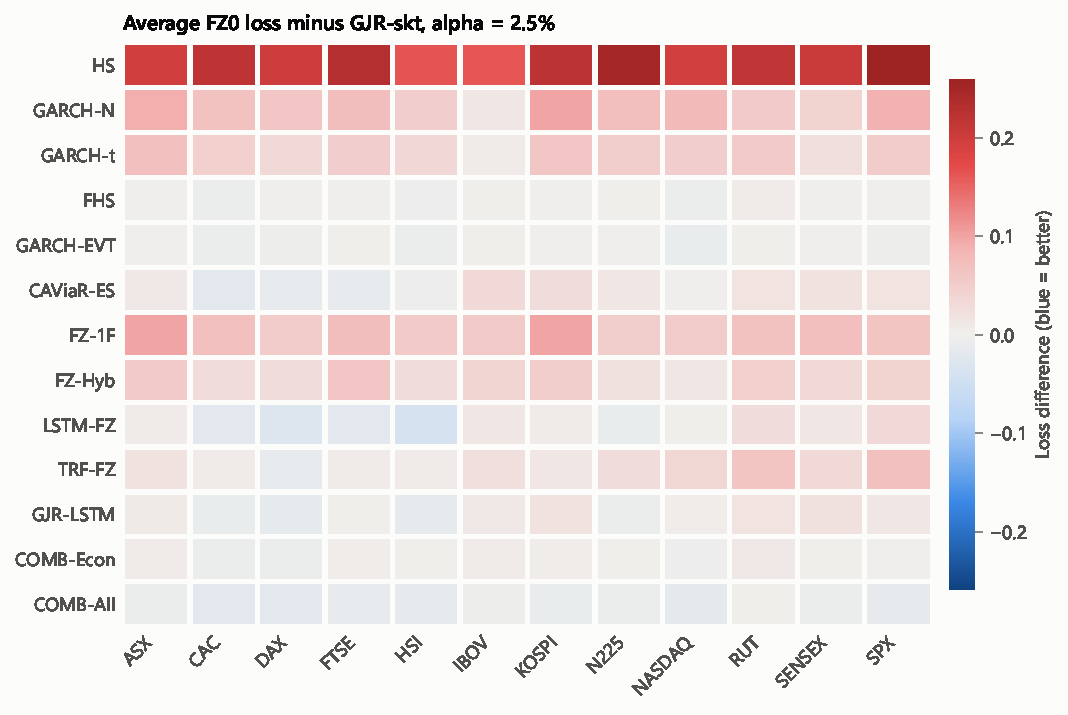
\includegraphics[width=\textwidth]{figures/heatmap_a025.pdf}
\caption{Average FZ0 loss difference from GJR-skt by asset, $\alpha=2.5\%$ (blue: lower loss).}\label{fig:heatmap}
\end{figure}

\subsection{Do the deep models add information?}
The cleanest test compares the two pre-specified combinations, which differ only in whether the three deep models are included. Table~\ref{tab:combo} shows that adding them lowers the loss at every risk level, with panel DM statistics between $-4.7$ and $-5.3$. The improvement is significant in 10 or 11 of the 12 markets and is never significantly negative. Figure~\ref{fig:combo} shows that the gain accumulates steadily over twenty years. It is not driven by a single episode: it is present before, during and after the global financial crisis and through the calm 2013--2019 period. A large part also comes after the COVID-19 shock. The deep models therefore contain information about tail risk that the econometric models, even averaged together, do not. This is our main finding. On their own the networks only match the best benchmarks, but they are \emph{complementary} to them.

\begin{table}[htbp]
\centering
\footnotesize
\caption{Value of adding the deep models to an econometric forecast combination}
\label{tab:combo}
\begin{tabular}{lrrrrr}
\toprule
Level & Loss diff & Panel DM t & p-value & \# assets better & \# assets worse \\
\midrule
1\% & -0.0168 & -4.73 & 0.000 & 10 & 0 \\
2.5\% & -0.0108 & -4.99 & 0.000 & 10 & 0 \\
5\% & -0.0080 & -5.25 & 0.000 & 11 & 0 \\
\bottomrule
\end{tabular}
\par\smallskip\parbox{\linewidth}{\scriptsize Loss difference COMB-All minus COMB-Econ (negative = adding the three deep models helps). The two combinations were specified before any results were seen and differ only by the inclusion of the deep models.}
\end{table}

\begin{figure}[htbp]\centering
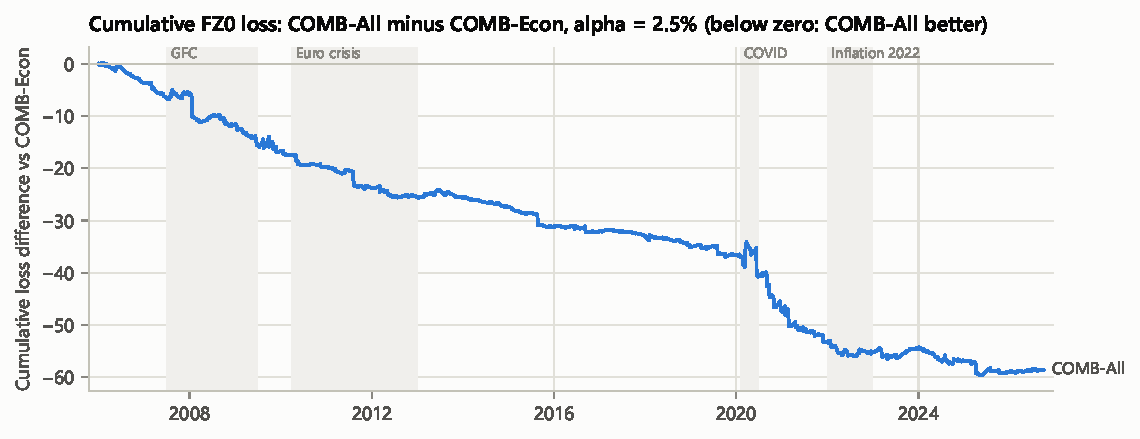
\includegraphics[width=\textwidth]{figures/cumulative_combo.pdf}
\caption{Cumulative FZ0 loss of COMB-All minus COMB-Econ (cross-asset average), $\alpha=2.5\%$. A downward slope means that adding the deep models to the combination lowers the loss.}\label{fig:combo}
\end{figure}

\subsection{Model confidence sets}
Table~\ref{tab:mcs} confirms the ranking. LSTM-FZ is the only single model contained in the 90\% MCS for all 36 asset--level combinations, and COMB-All is the only model in the pooled MCS with $p=1$ at every level. At $2.5\%$ the pooled MCS is $\{$COMB-All, LSTM-FZ, GJR-skt, FHS, GARCH-EVT$\}$. COMB-Econ has essentially the same average loss as GJR-skt yet is excluded from every pooled MCS. The reason is that its loss differential to COMB-All is small but extremely stable, so it is estimated very precisely.

\begin{table}[htbp]
\centering
\footnotesize
\caption{Model confidence set (90\%) membership}
\label{tab:mcs}
\resizebox{\textwidth}{!}{%
\begin{tabular}{lrrrrrr}
\toprule
Model & \# assets 1\% & \# assets 2.5\% & \# assets 5\% & Pooled p 1\% & Pooled p 2.5\% & Pooled p 5\% \\
\midrule
HS & 0 & 0 & 0 & 0.001 & 0.001 & 0.000 \\
GARCH-N & 1 & 1 & 1 & 0.001 & 0.000 & 0.000 \\
GARCH-t & 5 & 2 & 1 & 0.001 & 0.000 & 0.000 \\
GJR-skt & 12 & 11 & 11 & 0.299 & 0.166 & 0.328 \\
FHS & 12 & 11 & 11 & 0.169 & 0.174 & 0.281 \\
GARCH-EVT & 12 & 11 & 12 & 0.348 & 0.174 & 0.328 \\
CAViaR-ES & 12 & 12 & 11 & 0.009 & 0.035 & 0.328 \\
FZ-1F & 2 & 0 & 0 & 0.000 & 0.000 & 0.000 \\
FZ-Hyb & 6 & 1 & 0 & 0.005 & 0.000 & 0.000 \\
LSTM-FZ & 12 & 12 & 12 & 0.528 & 0.406 & 0.328 \\
TRF-FZ & 12 & 11 & 9 & 0.183 & 0.048 & 0.044 \\
GJR-LSTM & 12 & 10 & 12 & 0.057 & 0.035 & 0.126 \\
COMB-Econ & 8 & 6 & 5 & 0.001 & 0.000 & 0.000 \\
COMB-All & 12 & 12 & 12 & 1.000 & 1.000 & 1.000 \\
\bottomrule
\end{tabular}
}
\par\smallskip\parbox{\linewidth}{\scriptsize Columns '\# assets': number of assets whose MCS contains the model. 'Pooled p': MCS p-value on the cross-asset average loss series; a model is in the pooled MCS if p > 0.1. Range statistic, stationary bootstrap, 2000 replications.}
\end{table}

\subsection{Calibration}
Table~\ref{tab:bt_a025} reports absolute backtests. Accuracy and calibration rank models differently. GARCH-EVT and FHS are the best-calibrated models: their violation rates are within 0.1 percentage points of nominal, and they are rarely rejected by any VaR or ES test. The deep models are slightly less conservative, with violation rates of 2.79--2.80\% at the 2.5\% level. They are rejected more often by the coverage and calibration tests, and the Transformer is rejected by the dynamic-quantile test in all twelve markets. This indicates that its forecasts react too slowly to new information. All models have negative Acerbi--Szekely $Z_2$, i.e.\ a slight tendency to understate ES. The tendency is smallest for GARCH-EVT, FHS and COMB-All. COMB-All has a violation rate of 2.67\% and is rejected by the unconditional and conditional coverage tests in no market. The combination therefore inherits the accuracy of the deep models without their calibration weaknesses.

\begin{table}[htbp]
\centering
\footnotesize
\caption{Backtests, $\alpha=0.025$: number of assets (out of 12) rejecting at 5\%}
\label{tab:bt_a025}
\begin{tabular}{lrrrrrrrr}
\toprule
Model & Hit \% & UC & CC & DQ & ER & CCT-u & CCT-c & Z2 \\
\midrule
HS & 3.20 & 11 & 12 & 12 & 12 & 12 & 12 & -0.400 \\
GARCH-N & 3.68 & 11 & 11 & 12 & 12 & 12 & 12 & -0.652 \\
GARCH-t & 3.51 & 11 & 11 & 11 & 6 & 11 & 11 & -0.454 \\
GJR-skt & 2.72 & 2 & 3 & 3 & 2 & 2 & 3 & -0.114 \\
FHS & 2.60 & 0 & 1 & 1 & 2 & 0 & 0 & -0.067 \\
GARCH-EVT & 2.58 & 0 & 1 & 1 & 1 & 0 & 1 & -0.051 \\
CAViaR-ES & 2.73 & 3 & 2 & 5 & 5 & 4 & 1 & -0.133 \\
FZ-1F & 2.74 & 3 & 2 & 6 & 4 & 4 & 7 & -0.129 \\
FZ-Hyb & 2.74 & 2 & 2 & 3 & 5 & 5 & 2 & -0.135 \\
LSTM-FZ & 2.80 & 5 & 3 & 5 & 4 & 4 & 5 & -0.143 \\
TRF-FZ & 2.79 & 2 & 3 & 12 & 8 & 6 & 4 & -0.170 \\
GJR-LSTM & 2.79 & 5 & 6 & 6 & 4 & 5 & 4 & -0.155 \\
COMB-Econ & 2.78 & 4 & 3 & 4 & 3 & 3 & 3 & -0.143 \\
COMB-All & 2.67 & 0 & 0 & 4 & 4 & 1 & 3 & -0.095 \\
\bottomrule
\end{tabular}
\par\smallskip\parbox{\linewidth}{\scriptsize Hit \%: average violation rate (nominal 2.5\%). VaR tests: UC Kupiec, CC Christoffersen conditional coverage, DQ Engle--Manganelli. ES tests: ER McNeil--Frey exceedance residuals (one-sided bootstrap), CCT-u/CCT-c Nolde--Ziegel unconditional/conditional calibration. Z2: Acerbi--Szekely statistic averaged over assets (negative = ES too optimistic).}
\end{table}

\subsection{Crisis periods}
Table~\ref{tab:sub} and Figure~\ref{fig:cumdiff} show where the deep models gain and lose. LSTM-FZ accumulates a steady advantage over GJR-skt in calm and moderately volatile periods (2013--2019 and the euro-area crisis), and gives much of it back in a few days in March 2020. The COVID-19 crash was the fastest volatility increase in the sample, and GARCH-type recursions, which react to every squared return, adapted faster than networks trained on the previous eight years. The Transformer has its two largest losses in February 2018 (``Volmageddon'') and March 2020, both sudden volatility spikes. The hybrid, whose scale comes from GARCH, loses far less in March 2020 (0.12 against 0.35 for LSTM-FZ). None of the deep models' or combinations' crisis-period differences is significant at 5\%, because these windows are short. Figure~\ref{fig:episodes} illustrates the forecasts during the global financial crisis and the COVID-19 crash.

\begin{table}[htbp]
\centering
\footnotesize
\caption{Loss difference vs GJR-skt by subperiod, $\alpha=0.025$}
\label{tab:sub}
\begin{tabular}{lrrrrr}
\toprule
 & GFC & Euro crisis & COVID & Inflation 2022 & Calm 2013-2019 \\
\midrule
HS & 0.417 (3.3) & 0.278 (2.8) & 1.854 (1.6) & 0.170 (2.1) & 0.106 (2.7) \\
GARCH-N & 0.112 (2.5) & 0.056 (1.6) & 0.514 (1.6) & 0.106 (2.2) & 0.050 (2.6) \\
GARCH-t & 0.088 (2.3) & 0.048 (1.6) & 0.312 (1.3) & 0.064 (2.0) & 0.032 (2.2) \\
FHS & 0.005 (1.0) & -0.001 (-0.4) & -0.016 (-0.6) & -0.004 (-0.8) & 0.001 (0.5) \\
GARCH-EVT & 0.000 (0.0) & -0.001 (-0.3) & -0.012 (-0.4) & -0.005 (-0.9) & 0.002 (0.7) \\
CAViaR-ES & 0.037 (1.6) & 0.010 (1.3) & 0.264 (1.5) & -0.002 (-0.1) & -0.007 (-1.0) \\
FZ-1F & 0.096 (3.7) & 0.068 (3.4) & 0.457 (1.6) & 0.083 (2.7) & 0.056 (4.3) \\
FZ-Hyb & 0.073 (2.9) & 0.025 (1.7) & 0.406 (1.3) & 0.035 (1.3) & 0.033 (3.2) \\
LSTM-FZ & 0.013 (0.4) & -0.018 (-1.3) & 0.351 (0.9) & 0.011 (0.3) & -0.012 (-1.4) \\
TRF-FZ & 0.023 (0.7) & -0.001 (-0.1) & 0.626 (1.0) & 0.054 (1.6) & 0.016 (0.9) \\
GJR-LSTM & 0.039 (1.7) & 0.001 (0.2) & 0.121 (0.7) & 0.043 (1.4) & -0.004 (-0.8) \\
COMB-Econ & 0.009 (0.8) & 0.004 (0.5) & 0.110 (0.9) & -0.003 (-0.3) & 0.001 (0.2) \\
COMB-All & -0.008 (-0.9) & -0.007 (-0.8) & 0.072 (0.4) & -0.011 (-0.9) & -0.005 (-1.1) \\
\bottomrule
\end{tabular}
\par\smallskip\parbox{\linewidth}{\scriptsize Average FZ0 loss difference (negative = better than the benchmark); panel Diebold--Mariano t-statistic in parentheses.}
\end{table}

\begin{figure}[htbp]\centering
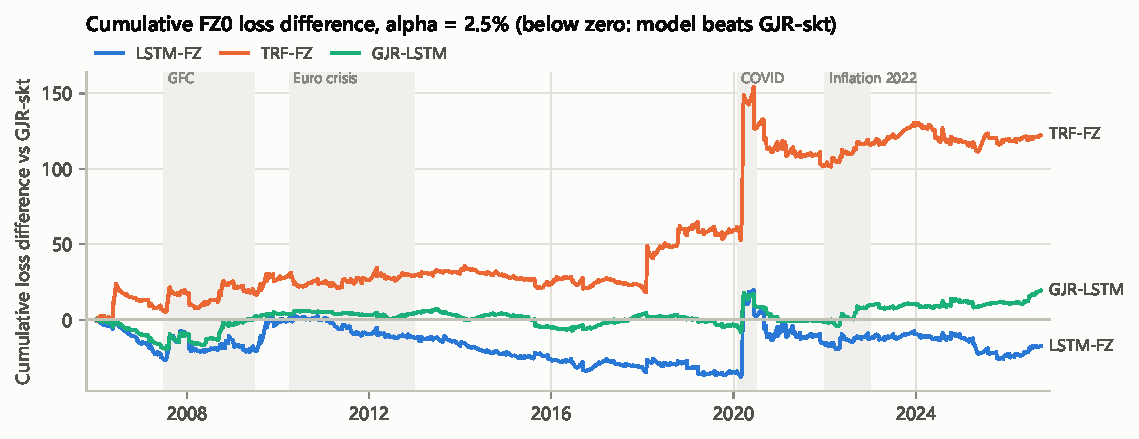
\includegraphics[width=\textwidth]{figures/cumulative_diff.pdf}
\caption{Cumulative FZ0 loss of each deep model minus GJR-skt (cross-asset average), $\alpha=2.5\%$. Shaded: crisis subperiods.}\label{fig:cumdiff}
\end{figure}

\begin{figure}[htbp]\centering
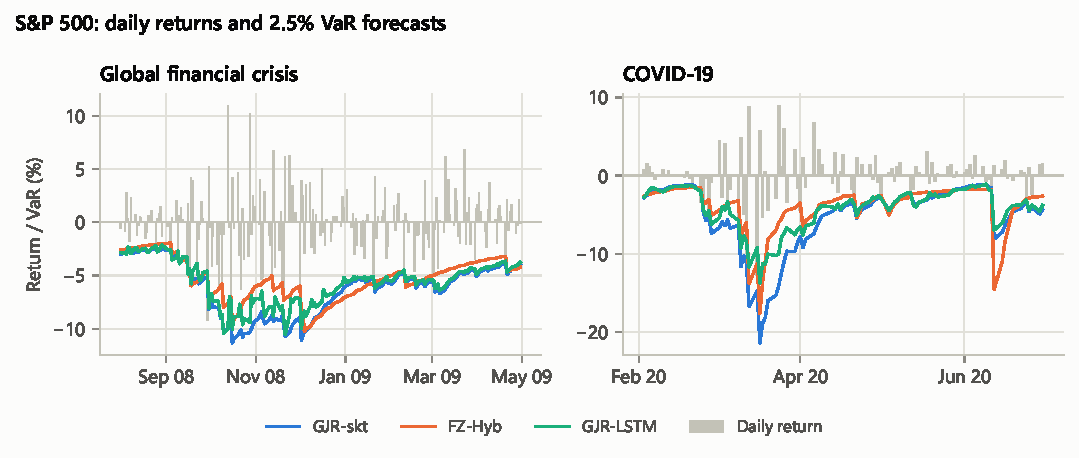
\includegraphics[width=\textwidth]{figures/episodes.pdf}
\caption{S\&P 500 daily returns and 2.5\% VaR forecasts of GJR-skt, FZ-Hyb and GJR-LSTM during the global financial crisis and the COVID-19 crash.}\label{fig:episodes}
\end{figure}

\subsection{A regulatory view}
Table~\ref{tab:reg} translates forecasts into the two quantities a bank cares about. The first is the level of the 97.5\% ES, the FRTB capital measure. The second is the Basel traffic light for 99\% VaR backtesting. GARCH-EVT is the most conservative model: it has the highest average ES and the fewest days in the yellow and red zones. COMB-All requires 2.2\% less capital than GJR-skt (3.17\% against 3.24\% of position value). Its traffic-light record is essentially identical (16.9\% against 16.7\% of days in the yellow zone, 0.24\% against 0.26\% in the red zone). The individual deep models need similar or slightly less capital (3.15--3.19\%), but they spend 2.5--3 times as many days in the red zone as GJR-skt.

\begin{table}[htbp]
\centering
\footnotesize
\caption{Regulatory view: capital and Basel traffic light}
\label{tab:reg}
\begin{tabular}{lrrr}
\toprule
Model & Capital (avg -ES 2.5\%) & Yellow zone \% days & Red zone \% days \\
\midrule
HS & 3.41 & 36.3 & 5.7 \\
GARCH-N & 2.78 & 51.1 & 6.0 \\
GARCH-t & 3.06 & 37.4 & 1.3 \\
GJR-skt & 3.24 & 16.7 & 0.3 \\
FHS & 3.26 & 18.9 & 0.2 \\
GARCH-EVT & 3.28 & 13.6 & 0.1 \\
CAViaR-ES & 3.18 & 20.6 & 2.4 \\
FZ-1F & 3.33 & 20.5 & 2.1 \\
FZ-Hyb & 3.24 & 18.8 & 0.9 \\
LSTM-FZ & 3.19 & 19.0 & 0.7 \\
TRF-FZ & 3.18 & 23.4 & 0.8 \\
GJR-LSTM & 3.15 & 23.6 & 0.6 \\
COMB-Econ & 3.17 & 18.7 & 0.5 \\
COMB-All & 3.17 & 16.9 & 0.2 \\
\bottomrule
\end{tabular}
\par\smallskip\parbox{\linewidth}{\scriptsize Capital: average forecast of $-\mathrm{ES}_{2.5\%}$ (FRTB measure), in \% of position value, averaged over assets. Traffic light: share of days on which the trailing 250-day count of 99\% VaR violations is 5--9 (yellow) or $\geq$10 (red).}
\end{table}

\subsection{What does the hybrid learn?}
Figure~\ref{fig:tail} plots the ES/VaR ratio implied by each model, a scale-free measure of tail heaviness. In GARCH-$t$ and GJR-skt it moves only through re-estimated shape parameters. Over 2006--2026 these drift upward from 1.25 to 1.35, as the rolling window absorbs more crash days. The hybrid's ratio is far more variable. It falls well below the parametric ratios during the calm 2012--2019 period, which means thinner standardised tails than the skewed-$t$ implies. It rises sharply after 2020 and stays above them during 2023--2024. The network therefore learns economically interpretable variation in tail shape. That this variation does not translate into significantly better forecasts suggests that, at a daily horizon and with returns alone, the predictable component of tail shape beyond volatility is small.

\begin{figure}[htbp]\centering
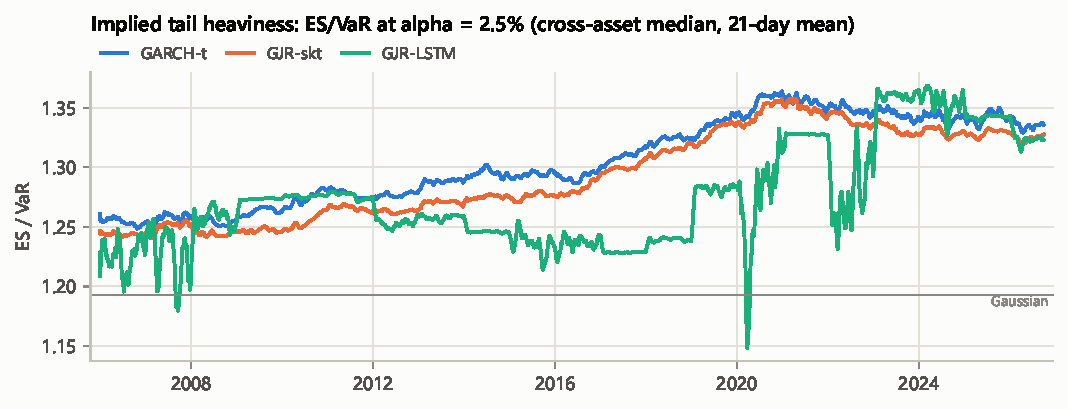
\includegraphics[width=\textwidth]{figures/tail_ratio.pdf}
\caption{Model-implied ES/VaR at $\alpha=2.5\%$ (cross-asset median, 21-day moving average). The grey line is the Gaussian value 1.193.}\label{fig:tail}
\end{figure}

\subsection{Robustness}
\paragraph{Seeds.} Table~\ref{tab:seeds} compares single networks with the three-seed ensembles. For LSTM-FZ, average losses across seeds differ by up to 0.007. That is larger than the differences among the four best models, so comparisons based on a single trained network would be unreliable. The ensemble is better than every individual seed for LSTM-FZ, and better than all but one for the other two models.

\paragraph{Specification revisions.} Two choices were revised after the first full run: the initialisation of the networks' output head and the optimiser for the semiparametric models (Appendix~\ref{app:v1}). Neither revision changes any conclusion. COMB-All is best, LSTM-FZ matches the top econometric models, and the FZ-GAS models underperform in both runs.

\begin{table}[htbp]
\centering
\footnotesize
\caption{Deep models: single seeds versus the seed ensemble, $\alpha=0.025$}
\label{tab:seeds}
\begin{tabular}{lrrrr}
\toprule
Model & Ensemble & Seed 0 & Seed 1 & Seed 2 \\
\midrule
GJR-LSTM & 1.1300 & 1.1336 & 1.1306 & 1.1297 \\
LSTM-FZ & 1.1244 & 1.1261 & 1.1251 & 1.1317 \\
TRF-FZ & 1.1497 & 1.1459 & 1.1656 & 1.1528 \\
\bottomrule
\end{tabular}
\end{table}
